\begin{homeworkProblem}[4]
\begin{enumerate}
% 4(a)
\item The relationship between $\lambda$ and $K$ is depicted below in Figure
\ref{fig:fig4a}.
\begin{SCfigure}[4][h]
    \centering
    \caption[The relationship between $\lambda$]{
        The relationship between $\lambda = \exp[r(1-N_t/K)]$ and $K$.
        $\lambda$, the population's growth rate, is described as a function of
        $K$. Here $K$ is selected to be $50$ and $r$ is selected to be $2$.
    }
    \label{fig:fig4a}
    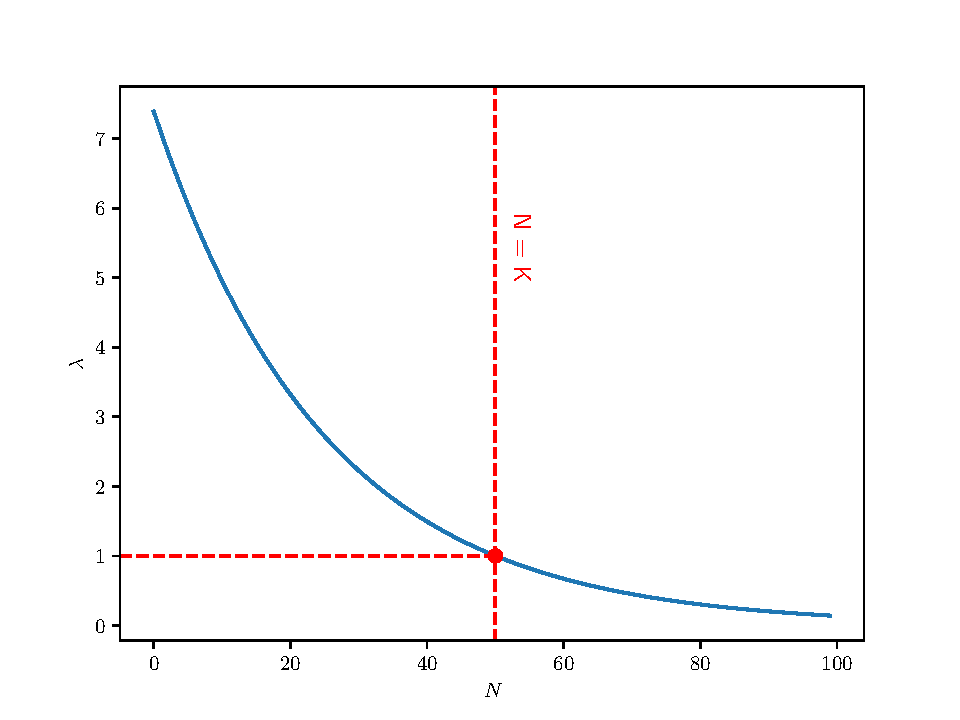
\includegraphics[scale=0.6]{../fig/fig4(a).pdf}
\end{SCfigure}
It's clear in Figure \ref{fig:fig4a} that $\lambda > 1$ when $N < K$, i.e., the
population can continue to grow and reproduce only if $N < K$.

% 4(b)
\item Plug in $\bar N = K$ into the equation, we'll have \[
    \begin{aligned}
        N_t &= \bar N = K,\\
        N_{t+1} &= N_t \exp[r(1-N_t/K)] = K \exp[r(1-K/K)] = K
    \end{aligned}
\]
Therefore, for $\bar N$ can make $N_{t+1} = N_t$ for two successive timepoints.
It is indeed the steady state.

% 4(c)
\item The condition of stability for the steady state depends on: \[
    \begin{aligned}
        &\left|\left.\derivlong[N]{N\exp[r(1-N/K)]}\right|_{\bar N}\right|\\
        &\qquad = \left| \left.\left(
            \frac{N^2 -rkN + N^2}{N^2} \exp[r(1-N/K)]
        \right)\right|_{\bar N} \right|\\
        &\qquad = |(2-r)e^r|
    \end{aligned}
\]
To make the steady state stable, we need \[
    |
    (2-r)e^r| < 1
\]
Solving this inequity gives \[
    \begin{aligned}
        &r < W_{-1}(-1/e^2) + 2\\
        &W(-1/e^2) + 2 < r < W(1/e^2) + 2
    \end{aligned}
\]
The approximate values are \[
    \begin{aligned}
        &r < -1.15\\
        &1.84 < r < 2.12
    \end{aligned}
\]
\pagebreak
% 4(d)
\item $r = 2, K = 2000$
\begin{figure}[h]
    \centering
    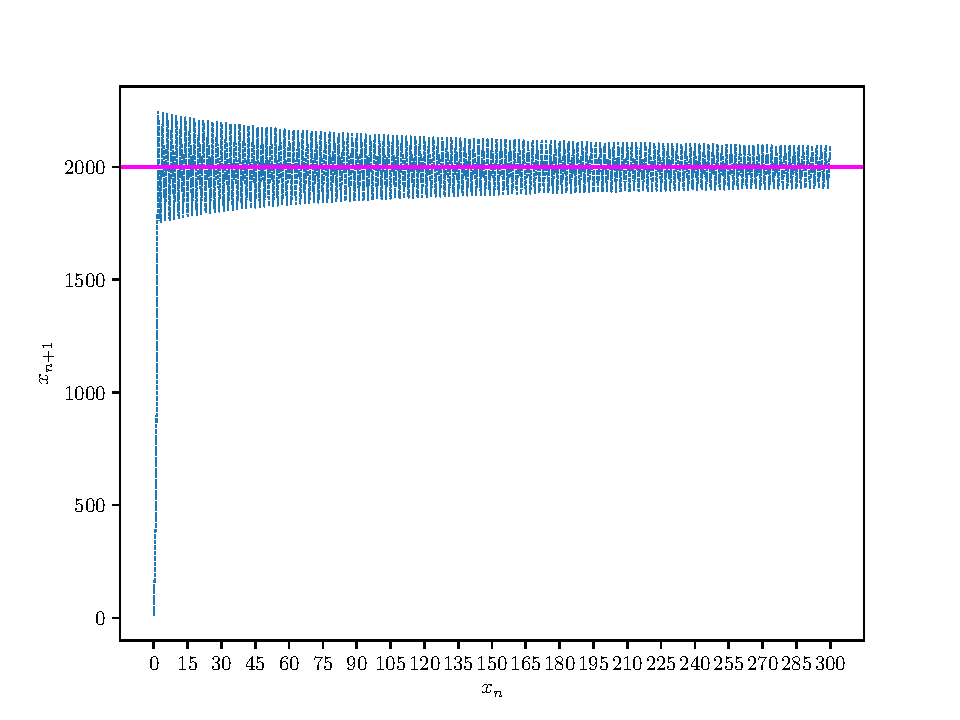
\includegraphics[scale=0.6]{../fig/fig4(d).pdf}
\end{figure}
\end{enumerate}
\end{homeworkProblem}